% Run pdfLaTeX twice from the repository root. Phase III vector figures live in results/.
\documentclass[10pt,a4paper]{article}
\usepackage[T1]{fontenc}
\usepackage[utf8]{inputenc}
\usepackage{tgpagella,tgcursor,amsmath}
\usepackage[margin=23mm,top=22mm,bottom=22mm,headheight=13pt]{geometry}
\usepackage{microtype,booktabs,tabularx,array,caption,fancyhdr,pgfplots}
\usepackage{graphicx}
\graphicspath{{results/phase3/cpu/figures/}{../results/phase3/cpu/figures/}}
\pgfplotsset{compat=1.17}
\usepackage[colorlinks=true,linkcolor=black,citecolor=teal!55!black,urlcolor=teal!55!black]{hyperref}
\hypersetup{pdftitle={The Cost of Exact Activation Counts in XLA},pdfauthor={FusionScope Project},
 pdfsubject={A compiler study of probe placement, reduction schedules, and model selection on CPU}}
\captionsetup{font=small,labelfont=bf,labelsep=period}
\pagestyle{fancy}\fancyhf{}
\fancyhead[L]{\small\itshape FusionScope}\fancyhead[R]{\small Exact activation counts in XLA}
\fancyfoot[C]{\small\thepage}
\renewcommand{\headrulewidth}{0.3pt}
\setlength{\parindent}{1em}
\setlength{\textfloatsep}{15pt plus 2pt minus 2pt}
\setlength{\emergencystretch}{1.5em}
\newcommand{\us}{\ensuremath{\,\mu\mathrm{s}}}
\newcommand{\V}[1]{\ensuremath{\mathrm{V}_{#1}}}
\newcommand{\Ecase}{\texttt{E3\_branch}}
\newcommand{\Ncase}{\texttt{N2\_branch}}
\newcommand{\artifact}[2]{\href{https://github.com/ZZzJunzum/Compiler_report/blob/e5964158e339cb1ff866b5f1ca4d0ba3bc9b6325/#1}{#2}}
\definecolor{measure}{HTML}{155968}
\definecolor{analytic}{HTML}{AF552C}
\definecolor{ridge}{HTML}{64488A}
\title{\bfseries The Cost of Exact Activation Counts in XLA\\[4pt]
       \large Probe Placement, Reduction Schedules, and Prospective CPU Selection}
\author{FusionScope Project}
\date{}

\begin{document}
\maketitle
\thispagestyle{plain}
\begin{abstract}
Returning two exact activation counts can change how a compiler computes the tensor that accompanies them. We study this cost in JAX/XLA on one Intel CPU. Across 32 synthetic workloads, all four pre-/post-ReLU placements produced the same optimized High Level Optimizer (HLO) computation within each workload. Changing the reduction schedule removed two 4\,MiB integer-mask exports in a million-element affine branch and gave a $3.07\times$ speedup. The analytic selector always chose joint reduction because its five cost coordinates favored that schedule in all 186 comparisons. We then crossed tile extent with observation strategy and tested a revised selector on 24 fresh conditions. The locked regression reduced geometric-mean execution latency by 13.9\% relative to fixed joint reduction (paired 95\% interval for the ratio, 0.797--0.943). Its largest gains came from row normalization. On four mixed-operator transfers its latency ratio rose to 1.047. A two-candidate timing policy selected within the repeatability floor of the fastest valid program on all 24 primary conditions. Setup costs changed the deployment result. Even with calibration reused, only two static choices and no two-candidate choices recovered their costs within 1,000 invocations.
\end{abstract}

\section{Introduction}
Suppose an inference service must return its usual tensor and the number of positive activations at two specified layers on every call. The two counters add only eight bytes to the logical output. Computing them can require scanning the entire activation domain, duplicating arithmetic or storing an intermediate across a fusion boundary. The choice that matters to the user is among programs that provide \emph{the same information}.

We examine two distinct compiler decisions. First, can a count move across a ReLU to an edge where the activation is already available? Second, if the compiler erases this source-level choice, can a different execution schedule share producer work or bound intermediate storage? Both questions have relevant precedents. Spartan adapts how often a training-time sparsity monitor runs~\cite{spartan}. SystemML optimizes materialization and shared aggregates~\cite{systemml}, and XTAT tunes XLA schedules and fusion decisions~\cite{xtat}. Here the sampling rate, two dependent observation sites and main output are fixed. Our experiment isolates the cost of fulfilling that contract.

The study makes three contributions. A placement control and a crossed ReLU-implementation control identify the source changes that survive compilation. A path-by-path HLO audit and a crossed experiment with tiled, unobserved controls measure how aggregation and tile extent interact. Finally, we explain a coefficient-independent restriction in a cost model and test a replacement selector on new input shapes, with separate accounting for the cost of choosing its schedule.

\section{Prior work}
Dong et al.\ quantify the cost of exhaustive activation-sparsity profiling in GPU training and use temporal adaptation to reduce its frequency~\cite[Table~7]{spartan}. Our observer must execute on each input. Boehm et al.\ show how shared aggregates benefit from common input scans and how producer duplication competes with materialization~\cite[Fig.~1 and Sec.~4.2]{systemml}. In our workload one observed layer feeds the next, and both counts accompany a full tensor output. XTAT discusses the replication of a producer across consumers with different iteration spaces~\cite{xtat}. These mechanisms motivate following the actual operands on all three output paths.

Halide makes computation and storage granularity explicit in a schedule~\cite{halide}. The oneDNN Graph Compiler distinguishes the size of a slice, its invocation count and total element accesses at a CPU fusion point~\cite[Fig.~3]{onednn}. Dodovi\'c et al.\ vary the reduction strategy for fused CUDA map--reduce kernels~\cite[Sec.~4.4]{cuda}. These studies motivate the tile sweep and help explain why a working-set proxy alone is incomplete. Our analytic equation borrows the maximum of compute and transfer time from the Roofline model~\cite{roofline}. Kaufman et al.\ evaluate learned models for TPU tiling and fusion, and TpuGraphs records configuration-specific runtimes for complete tensor graphs~\cite{kaufman,tpugraphs}. Those studies establish prior art for learned configuration selection. Our test concerns transfer across CPU workload families under an exact-observation contract.

\section{Experimental design}
\paragraph{Observation and inputs.}
For layer $i$, let $a_i=\max(z_i,0)$ and $q_i=\sum_j\mathbf{1}[a_{ij}>0]$. On finite inputs the predicate has the same value before and after the ReLU. The target program returns $(y,q_1,q_2)$. Single-counter controls in Phase I return only the requested count alongside $y$. Inputs are FP32, weights are fixed across input seeds, and counts fit in signed 32-bit integers. For each candidate we check finite, same-shaped FP32 $y$ against the unobserved program under the registered family tolerance. Both scalar integers must exactly match independent host counts from a diagnostic program that returns the preactivations. Three input seeds are validated and one fixed seed is timed.

\paragraph{Workloads.}
Each synthetic program has two ReLU sites. The elementwise family (E) uses affine transformations, the dense family (M) uses matrix products, and the normalization family (N) uses row-wise root-mean-square normalization with an affine transform. The convolution family (C) uses same-padded convolutions with a residual addition. A chain reads out the last activation. A branch additionally reads out a scaled copy of the first. In Phases I and II, four sizes and two topologies give eight conditions per family. Vector widths are 256, with up to 4,096 rows for E, 256 for M, and 1,024 for N. C uses $32\times32$ images with 16 channels and batches of 1, 4, 8 or 16. Two additional workloads use one or two adjacent blocks of the official Flax ResNet implementation, with input $1\times56\times56\times64$, fixed initialized weights, and inference-mode batch normalization.

\paragraph{Interventions.}
Phase~I crosses the two positions (pre or post) at each site, alongside four single-site variants and the unobserved baseline. This gives $32\times9=288$ synthetic configurations and 18 external configurations. Phase~II fixes both sites after the ReLU and varies scheduling (Table~\ref{tab:strategies}). E, M and N are tiled only across whole rows and C across whole images. Every legal registered tile size is measured, including one-tile controls. The 32 conditions yield 250 configurations including 32 baselines and 122 tiled implementations. The batch-one external workloads contribute eight more configurations.

\begin{table}[htbp]\centering\small
\caption{Execution strategies in Phase II. All observed strategies retain the same $y$ and both counts.}\label{tab:strategies}
\begin{tabularx}{\linewidth}{@{}l l X@{}}\toprule
ID & Strategy & Execution boundary\\\midrule
\V{0} & Unobserved & Return $y$ only. Reference for incremental observation cost.\\
\V{1} & Separate counts & Two mask-to-integer reductions inside one compiled program.\\
\V{2} & Joint reduction & A variadic \texttt{lax.reduce} combines two masks using componentwise integer sums.\\
\V{3} & Materialized stage & The first executable returns $(a_1,q_1)$. A second consumes $a_1$ and returns $(y,q_2)$.\\
\V{4}$(b)$ & Tiled partial sums & A \texttt{lax.map} body produces a tile of $y$ and two partial sums. Combine the tiles and sum the partials.\\
\bottomrule\end{tabularx}\end{table}

\paragraph{Measurements and comparisons.}
We used JAX and jaxlib 0.9.0.1 on an Intel Core i5-13420H with each process pinned to one logical CPU. Inputs were device-resident. Compilation and lowering were timed separately. Each candidate block used six warm-up rounds and twenty timed rounds in randomized order, waiting for the entire output tree on every call. Discovery used five independent processes and confirmation used three new processes. Each external workload used five. Phase~II also screened five fixed cases in three processes before expanding the matrix. It recorded 43,380 formal candidate calls, 44,960 A/A calls and 6,507 successful configuration--seed--process checks, including baseline checks. A further clean-clone screening replay is reported separately.

For condition $c$ and schedule $v$, $T_{cv}$ is the median of process medians. Speedup is the median of within-process $t_1/t_v$. We report selection regret as $T_{c,\mathrm{selected}}/\min_{v\ne0}T_{cv}-1$ over valid observed candidates. For Phase~II, four aliases each call the same \V{0} or \V{1} executable. The larger of the two empirical 95th percentiles of absolute within-process differences between alias medians gives the A/A floor. A speed change must exceed that floor and agree in direction across a strict majority of processes. A decision is within the floor when its gap to the best median is no larger than the floor. The two summaries aggregate in different orders. The floor describes local repeatability and does not constitute a confidence interval.

\section{How the observation changes the program}
\subsection{Probe placement often disappeared during optimization}
In every synthetic condition the four double-site placements shared one normalized optimized-HLO fingerprint. No fastest-versus-runner-up order was resolved in independent confirmation. Observing still cost time. The median paired latency ratio to the unobserved baseline across 128 double-site configurations was 1.107, and a clean full replay gave 1.110. Across both runs all 306 synthetic and external configuration fingerprints matched. The placement model's median regret was 0.956\%, versus 0.749\% for always observing after both ReLUs. Their small ordering reversed on replay (0.699\% versus 0.872\%). Those differences provide little evidence for distinct placement costs.

Each external ResNet condition retained four fingerprints, although its latency order remained unresolved. A separate compile-and-validate control crossed the ReLU expression with workload on one small affine graph and one ResNet block. Direct \texttt{maximum} produced one fingerprint per graph across placements, while \texttt{jax.nn.relu} produced four. This identifies a source-level condition sufficient to change the observed equivalence in these two cases. It leaves the responsible pass and machine-code equivalence open.

The single-site controls also allow an interaction estimate, $I=t_{12}-t_1-t_2+t_0$. Here $t_1$ and $t_2$ refer to observing just one site each. In both topologies of the largest normalization workload, all four two-site placements had a negative interaction beyond the registered A/A pseudo-interaction threshold in discovery and confirmation, in both full runs. These eight configurations show that adding the two measured single-site overheads can overstate the joint cost even when all four placements compile alike.

\subsection{A producer can reappear along three output paths}
We trace $y,q_1,q_2$ separately from the HLO entry tuple, binding each fusion-body parameter at its call site. A duplicate requires the same tagged source scope, opcode, type and shape, attributes, and recursively matched operands in distinct invocation groups. References to one computed value count once. This conservative match can miss algebraically equivalent rewrites. On \Ecase{} ($4096\times256$), the first affine add appears at lines 72, 93 and 107 of the archived \V{1} HLO, along $q_2,q_1,y$ respectively. Two separate reduction trees shrink the count domains through $128\times8$ and $4\times1$ to scalars. Table~\ref{tab:audit} gives controls from the other families.

\begin{table}[htbp]\centering\small
\caption{Extra copies of tagged arithmetic expressions in five audited HLO modules. The last column counts complete int32 mask outputs crossing a fusion boundary under separate counting.}\label{tab:audit}
\begin{tabular}{@{}lrrr@{}}\toprule
Condition & Copies with $y$ only & Copies with counts & Exported mask size\\\midrule
E0 chain & 0 & 7 & 32 KiB\\
E3 branch & 0 & 7 & 8 MiB\\
M3 chain & 0 & 2 & 512 KiB\\
N3 chain & 4 & 14 & 2 MiB\\
C3 chain & 0 & 3 & 0\\
\bottomrule\end{tabular}\end{table}

For \Ecase{}, buffer assignment places two 4\,MiB int32 masks at offsets 0 and 4,194,304 in the same temporary allocation. Both optimized LLVM kernels contain vector int32 stores. This establishes emitted stores to allocated buffers. Cache service and physical DRAM traffic were unmeasured. In C3 the mask conversion already resides in a reduction fusion, so the same source expression produces no complete mask export.

\subsection{Removing a full mask and removing arithmetic have different effects}
On \Ecase{}, the joint reduction eliminated both complete mask exports and reduced the compiler's temporary allocation from 8,392,704 to 16 bytes. Tagged arithmetic copies fell from seven to five. Independently confirmed speedup over separate counts was $3.07\times$ and the median paired saving was $3,747\us$, above the $1,150\us$ floor. Tiling by 16 also removed both full-size exports, but its loop body still exported 32\,KiB of mask data per invocation. It retained seven duplicate sites and an estimated 6,291,456 excess simple scalar arithmetic operations across tiles, versus 4,194,304 for the joint reduction. Its speedup was $1.86\times$. Explicitly transmitting the first activation in \V{3} used two calls and achieved $0.81\times$.

On the large convolution chain a batch tile of two achieved $0.43\times$ the speed of separate counts. Its eight smaller convolution batches change both loop scheduling and kernel shape. On the two external ResNet graphs, joint reduction's paired savings (788 and $865\us$) fell below their respective A/A floors (927 and $1,823\us$). A clean clone reproduced all 43 screening configuration fingerprints and passed another 387 output checks. It measured $2.92\times$ for joint reduction on \Ecase{} and $0.42\times$ for the two-image convolution tile.

\begin{table}[htbp]\centering\small
\caption{Independent confirmation by family. The middle column counts paired improvements of joint over separate counts beyond the A/A floor. No joint-reduction slowdown met the same rule. The last four columns count the schedule with the smallest cross-process median, including unresolved differences.}\label{tab:families}
\begin{tabular}{@{}lrrrrrr@{}}\toprule
 & & & \multicolumn{4}{c}{Fastest observed schedule}\\\cmidrule(l){4-7}
Family & Cases & Resolved gains & Separate & Joint & Staged & Tiled\\\midrule
Elementwise   & 8 & 6 & 0 & 5 & 0 & 3\\
Dense         & 8 & 0 & 2 & 2 & 0 & 4\\
Normalization & 8 & 5 & 0 & 0 & 0 & 8\\
Convolution   & 8 & 0 & 2 & 1 & 1 & 4\\
\bottomrule\end{tabular}\end{table}

Normalization explains why separate counts are too weak a baseline for assessing a selector. Joint reduction improved on them beyond the noise floor in five of eight conditions. Yet a tiled schedule had the lowest median in all eight (Table~\ref{tab:families}). Thus a model can identify an improvement to the original instrumentation and still miss the fastest implementation of the same query.

\section{Why cost prediction failed to improve on fixed joint reduction}
All selection scores were locked before independent confirmation. Each fold excluded an entire family, including every size, topology and tile. External scores used training data from the four synthetic families only. Both selectors used the unobserved program's optimized HLO, tensor shapes and the declared schedule. Compiled candidate IR was reserved for subsequent explanation. For 16 of 34 synthetic and external baseline graphs, at least one ReLU anchor was missing or ambiguous. A missing anchor contributed an empty producer slice, and ambiguous anchors used the largest local producer slice.

\begin{table}[htbp]\centering\small
\caption{Held-out selection on 32 synthetic conditions. The reference in each row is the fastest valid observed schedule. Fixed tile uses the largest legal tile of at most 16. Discovery tile uses a separately timed search.}\label{tab:regret}
\begin{tabular}{@{}lrrrrr@{}}\toprule
Policy & Median regret & P90 regret & Within A/A & Exact best & MAE (\(\mu\)s)\\\midrule
Fixed separate counts & 63.9\% & 203.2\% & 11 & 4 & ---\\
Fixed joint reduction & 10.9\% & 95.4\% & 19 & 8 & ---\\
Fixed tile & 11.5\% & 87.9\% & 20 & 9 & ---\\
Analytic selector & 10.9\% & 95.4\% & 19 & 8 & 1,336.3\\
Ridge selector & 31.0\% & 98.4\% & 13 & 5 & 691.6\\
Discovery tile & 0.0\% & 55.1\% & 26 & 18 & ---\\
\bottomrule\end{tabular}\end{table}

\paragraph{The analytic choice is forced.}
The analytic model combines host call count $H$, estimated arithmetic $F$, a transfer proxy $B$, reduction levels $L$ and loop steps $S$ in Eq.~\eqref{eq:cost}.
\begin{equation}
 \widehat T = dH+\max(fF,bB)+rL+sS,\qquad d,f,b,r,s>0 .
 \label{eq:cost}
\end{equation}
We audited the frozen inputs to Eq.~\eqref{eq:cost} after confirmation. The 218 observed synthetic candidates include 32 joint schedules and 186 alternatives. For \emph{every} within-condition alternative, all five coordinates are greater than or equal to those of the joint schedule, and the reduction-level estimate is at least two levels higher. The maximum and the sum are coordinatewise nondecreasing. Since $r>0$, the complete prediction is strictly higher for every alternative, regardless of the fitted coefficient values. This is a property of the registered feature rows and equation. Consequently, although the analytic selector reduced median regret from 63.9\% for fixed separate counts to 10.9\%, its choices coincide with fixed joint reduction on all 32 synthetic graphs.

One cause is visible in the feature definitions. \V{2} is assigned zero exported-mask capacity, one reduction tree, one host call and no loop. The proxy charges other schedules for buffers, levels or loops, but offers a tile little credit for improving locality or the throughput of a row kernel. The estimated footprint also assumes two full masks for \V{1} even on C3, where the compiled program exports none. Adjusting coefficients alone cannot repair the ordering proved above.

\paragraph{Lower absolute error coexisted with worse decisions.}
Ridge used standardized log-transformed features, a fixed penalty of one, and a target of $\log(t_v/t_0)$. MAE in Table~\ref{tab:regret} averages per-candidate median absolute error over 218 candidates. Ridge predictions are multiplied by the measured baseline time to express errors in microseconds. The baseline factor cancels when selecting a schedule. Ridge changed the fixed joint choice in 12 conditions. In confirmation two changes lowered median latency and ten raised it. Of those 12 differences between cross-process medians, two gains and six losses exceeded the A/A floor.

Two diagnostics expose what the fitted model can represent. Graph-only features enter additively and cancel in a within-graph score difference. In the held-out dense, normalization and convolution folds, respectively, the training graphs all had zero baseline dot, reduction and convolution sites for the corresponding feature. A family-specific interaction between such an operation and tile size is difficult to learn from these folds. A second check compares 24 one-tile schedules whose complete normalized HLO equals that of separate counts. Ridge assigned them a median absolute predicted relative difference of 7.9\% from the equivalent separate-count program. Sixteen of the 24 predictions differed by over 5\%. Neither diagnostic alone establishes a hardware cause.

\begin{figure}[htbp]\centering
\pgfplotsset{caseaxis/.style={width=.48\linewidth,height=4.4cm,scale only axis=false,
 xmin=-.15,xmax=4.15,ymin=.4,ymax=2.65,xtick={0,1,2,3,4},xticklabels={1,4,16,64,256},
 ytick={.5,1,1.5,2,2.5},xlabel={Rows per tile},grid=major,grid style={black!9},
 tick label style={font=\scriptsize},label style={font=\small},title style={font=\small\bfseries},
 every axis plot/.append style={line width=0.95pt,mark size=1.8pt}}}
\begin{tikzpicture}
\begin{axis}[caseaxis,title={Elementwise branch, $4096\times256$},ylabel={Tile time / joint time}]
\addplot[gray,densely dotted,no marks] coordinates {(0,1)(4,1)};
\addplot[measure,mark=*] coordinates {(0,2.558)(1,1.698)(2,1.634)(3,1.642)(4,2.217)};
\addplot[analytic,dashed,mark=square*] coordinates {(0,2.313)(1,1.330)(2,1.090)(3,1.051)(4,1.127)};
\addplot[ridge,dashdotted,mark=triangle*] coordinates {(0,1.060)(1,1.067)(2,1.036)(3,1.032)(4,1.049)};
\end{axis}\end{tikzpicture}\hfill
\begin{tikzpicture}
\begin{axis}[caseaxis,title={Normalization branch, $256\times256$},
 legend style={font=\scriptsize,draw=none,fill=white,at={(.5,1)},anchor=north,legend columns=3,
 column sep=1pt},legend cell align=left]
\addplot[gray,densely dotted,no marks,forget plot] coordinates {(0,1)(4,1)};
\addplot[measure,mark=*] coordinates {(0,.999)(1,.787)(2,.511)(3,1.804)(4,1.401)};\addlegendentry{CPU}
\addplot[analytic,dashed,mark=square*] coordinates {(0,2.277)(1,1.339)(2,1.166)(3,1.374)(4,2.426)};\addlegendentry{Analytic}
\addplot[ridge,dashdotted,mark=triangle*] coordinates {(0,1.339)(1,1.235)(2,1.138)(3,1.086)(4,1.157)};\addlegendentry{Ridge}
\end{axis}\end{tikzpicture}
\caption{Each series is normalized to its own joint-reduction value. Below one, tiling wins. CPU points use ratios of confirmation medians. The two prediction curves use locked scores. These cases illustrate a correct and a missed joint-versus-tile decision.}\label{fig:rank}
\end{figure}

On \Ncase{}, a 16-row tile took $184.15\us$ and the joint schedule took $360.10\us$, a gap above the $101.44\us$ A/A floor. Both models predicted the tile to be slower (Fig.~\ref{fig:rank}). Conversely, on the small E1 chain, ridge preferred a one-row tile over the joint reduction by about 3\% of predicted latency. It took $138.05\us$ versus $59.15\us$ in confirmation. Fixed joint and fixed tile in Table~\ref{tab:regret} already exploit different regimes. A separate discovery sweep picked a tile within the A/A floor of the best observed schedule on 26/32 conditions, but paid to compile and time all legal tiles.

\section{Prospective selection on new workloads}
\label{sec:prospective}
We used the 32 previously measured conditions for development. We crossed tile extent with three observer settings on four old graphs. We also timed separate and variadic joint counts at every legal tile on the complete development grid. A tile contains complete rows or convolution samples, preserving the normalization domain and spatial halo. The staged schedule still invokes two executables. A main-only tiled control isolates changes in the unobserved computation.

For extent $b$, let $t_0(b)$, $t_s(b)$ and $t_j(b)$ be process medians for the main computation alone, separate counts and joint counts. We estimated each observer's cost relative to its own $t_0(b)$. For the interaction we estimated $[t_s(b)-t_j(b)]-[t_s(B)-t_j(B)]$, where $B$ is the full batch. Four aliases of the same executable supplied balanced pseudo-interactions. Six of eight nontrivial interactions exceeded the corresponding 95th-percentile floor and had the same sign in all five processes. On the affine branch the 16-row interaction was $-1{,}856\us$ against a $590\us$ floor. Separate counting exported 8\,MiB of full masks at whole extent and 32\,KiB per iteration at 16 rows. The two mask volumes accumulated over all 256 iterations are equal. The compiler allocated and scheduled them at different extents. Neither convolution interaction cleared its floor.

\begin{figure}[htbp]\centering
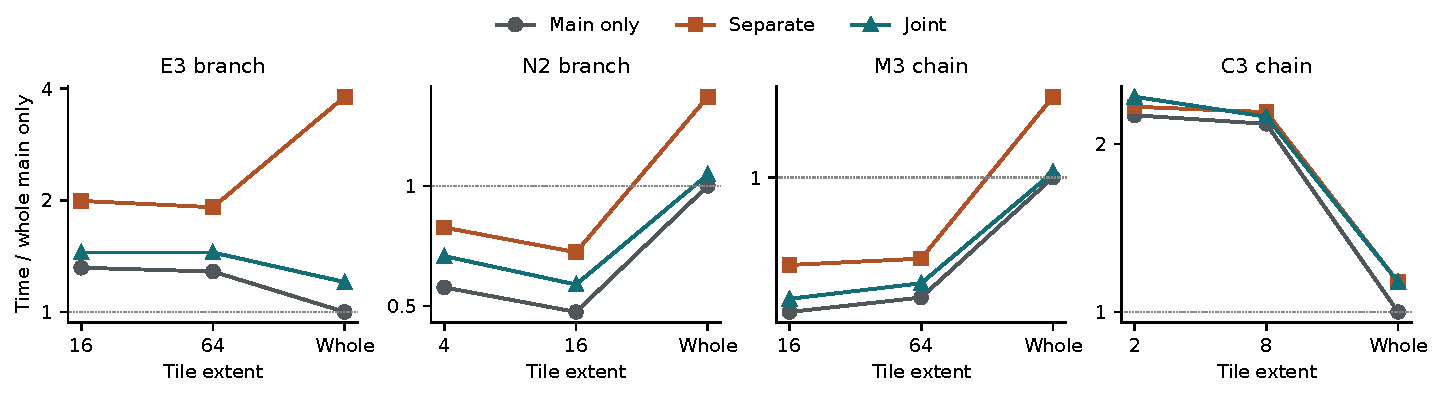
\includegraphics[width=\linewidth]{mechanism.pdf}
\caption{Matched main-only, separate and joint schedules on the four mechanism workloads. The denominator in each panel is that workload's whole-extent, main-only time. The vertical axis uses a logarithmic scale.}\label{fig:cross}
\end{figure}

\paragraph{Selection and independent measurements.}
The revised analytic model separates live capacity, accumulated visits, stage materialization and loop trips. A pinned copy sweep estimated a 2\,MiB change point in effective bandwidth. Development-shape single-layer measurements supplied the nearest measured dense or convolution throughput in log-shape distance. We compared the revised analytic models with log-latency regression and pairwise logistic ranking, each with and without operator and tile interactions. Entire graph families were held out in the outer folds. Inner training-family folds selected the regularization penalty. Mean outer-fold log regret selected the regression with interactions (0.0254, versus 0.1996 without interactions). The interaction ranker (0.0452) supplied the shortlist alternative.

The four families each supplied three new sizes and two topologies. Affine, dense and normalization inputs were $32\times192$, $128\times320$ and $512\times640$. Convolution used NHWC shapes $(2,24,24,24)$, $(4,40,40,32)$ and $(8,48,48,48)$. Four further chain graphs used both dense--normalization orderings at $32\times320$ and $512\times192$. Legal row tiles divided the batch and came from $\{1,4,16,64,256,B\}$. Convolution used $\{1,2,4,8,16,B\}$. The 28 graphs had 368 configurations, including 28 unobserved controls. The static lock fixed all choices before any new observed executable was compiled. Two independently funded discovery policies each tested joint counting and one alternative in two fresh processes. Each policy used six warm-ups, eight timed rounds and a joint-count A/A block per process. A second lock froze their decisions before a five-process exhaustive confirmation with six warm-ups, 30 interleaved rounds and three separate A/A blocks per graph. Input seeds and weights differed from development. We checked finite FP32 tensors and exact integer counts on three seeds.

\subsection{Confirmation and deployment cost}\label{sec:budget}
All 5,520 configuration--seed--process checks in independent confirmation passed. The primary endpoint gives each of the 24 graphs equal weight. Within a graph we take the median of the five selected-to-joint latency ratios. Their geometric mean was 0.861. A 10,000-draw bootstrap resampled sizes within each family, kept both topologies in each size block, and resampled the same process indices for the two schedules within a graph. The 95\% interval was $[0.797,0.943]$. The prespecified tests required a ratio at most 0.95, an upper bound below 1 and a P90 regret at most two percentage points above fixed joint. All three criteria were met. Omitting an entire size level across families gave ratios from 0.815 to 0.901.

\begin{table}[htbp]\centering\small
\caption{Independent confirmation on 24 primary graphs. Regret is the chosen cross-process median divided by the fastest valid observed median, minus one. A/A counts choices whose paired gap from that fastest schedule is inside the measured floor. The oracle is an in-sample reference bound.}\label{tab:fresh}
\begin{tabular}{@{}lrrrr@{}}\toprule
Policy & Time / joint & Median regret & P90 regret & Within A/A\\\midrule
Fixed joint                   & 1.000 & 1.4\% & 100.9\% & 16\\
Fixed separate-count tile     & 0.981 & 14.9\% & 50.1\% & 3\\
Revised analytic, kernel rates& 0.922 & 1.2\% & 75.5\% & 16\\
Locked static regression      & 0.861 & 4.4\% & 15.3\% & 14\\
Time joint and fixed tile     & 0.871 & 1.4\% & 19.4\% & 17\\
Time joint and ranked alternative & 0.824 & 0.0\% & 2.2\% & 24\\
Valid oracle                  & 0.820 & 0.0\% & 0.0\% & 24\\\bottomrule
\end{tabular}
\end{table}

The static rule changed 20 decisions. Eight were faster and 12 were slower in paired process medians, with eight gains and ten losses exceeding their own A/A floor. The geometric mean reflects the magnitudes of those changes. The family ratios were 0.823 (affine), 1.077 (dense), 0.598 (normalization) and 1.039 (convolution). On the $32\times192$ affine branch a 16-row joint tile took $36.20\us$ against $78.85\us$ for whole joint. On the $128\times320$ dense branch a 64-row joint tile took $669.50\us$ against $561.40\us$. On four mixed transfers, the static and timed-shortlist ratios were 1.047 and 0.947, respectively. These four graphs were excluded from model selection and from the primary endpoint.

The revised analytic coordinates made joint reduction dominate all alternatives on only two development graphs and zero primary graphs. Allowing rank reversals did not identify every useful tile. Adding calibrated layer throughput to the capacity-and-visits model moved its primary ratio from 0.916 to 0.922. Adding interactions to log regression moved the ratio from 0.904 to 0.861. For the pairwise objective, the corresponding ratios were 0.860 and 0.859. These are secondary comparisons of the frozen models. The original analytic and ridge models covered 162 of 288 observed primary candidates. Both had zero median regret against the common-domain oracle. The expanded grid exposed faster alternatives on individual graphs.

\begin{figure}[htbp]\centering
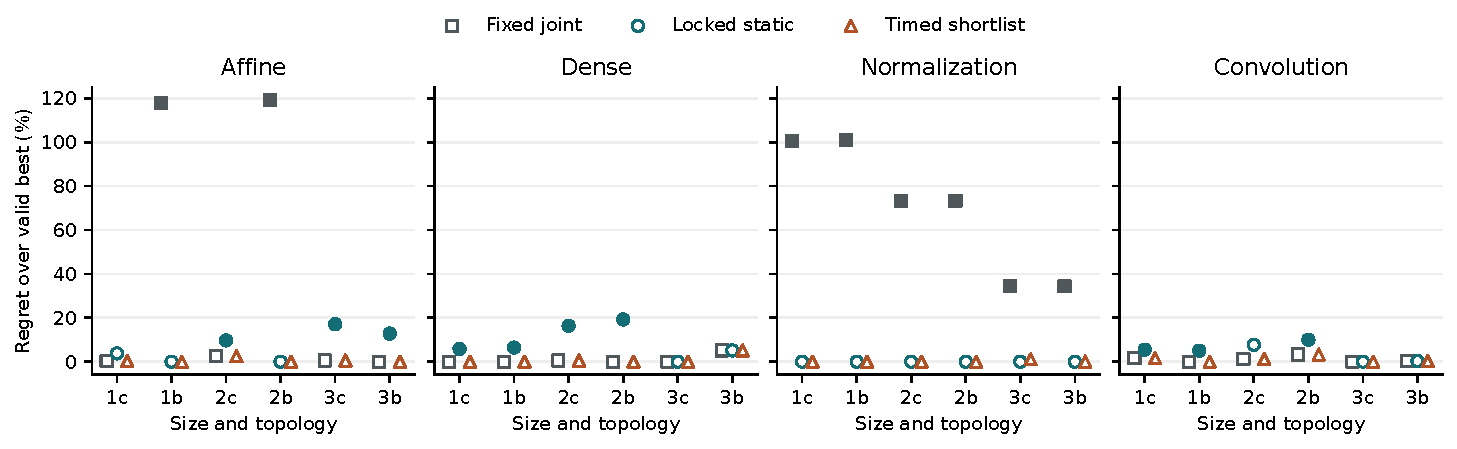
\includegraphics[width=\linewidth]{regret.pdf}
\caption{Regret on each fresh primary graph. An open marker denotes a gap inside the empirical A/A floor. The letters c and b denote chain and branch. Some markers coincide near zero.}\label{fig:regret}
\end{figure}

Both full-extent tile controls matched their direct counterpart's normalized HLO on every new graph (56/56). All 56 timing differences were unresolved. A diagnostic that compiled all observed candidates and chose the earliest representative of the frozen choice's equivalent HLO class yielded the same primary latency ratio (0.861) at a median reused setup of 1.58\,s. A clean checkout reproduced all 36 mechanism fingerprints and passed 540 more output checks. A separate Windows profiling run on the affine branch measured median process-cycle counts of 9.61 million for separate counts and 3.55 million for joint counts. At 16 rows these counts were 5.28 and 4.05 million, respectively. These totals cover all threads of the pinned process.

\paragraph{Paying for selection.}
For $H$ invocations we charged $C_p+H T_p$. The setup term includes any baseline extraction, feature scoring, compilation and exploratory blocks required by policy $p$. Both timed policies paid for both candidate compilations, warm-ups and A/A trials in each of their two discovery processes. The retained executable can serve subsequent invocations. Cold startup assigns the entire 714\,ms device calibration to the first deployment. Reuse assigns zero additional calibration cost. Offline model training and common framework initialization are outside these totals.

With reused calibration, the median setup was 151\,ms for static selection and 606\,ms for the learned shortlist. At $H=1{,}000$ the respective median total-time ratios to fixed joint were 1.27 and 1.75. Static selection broke even by 1,000 calls on two primary graphs. In the eight cases with positive per-call savings, the first non-worse horizon ranged from 569 to 3,408 calls (median 1,884). The learned shortlist improved eight decisions and retained joint counting on the other 16. Its corresponding horizons were 3,078--12,197 calls. With cold calibration none of the three adaptive comparisons in Fig.~\ref{fig:reuse} beat fixed joint by 1,000 calls on any primary graph. At 1,000 calls the learned shortlist's median paired total-time ratio to the equally funded fixed-tile shortlist was 0.991 with reused calibration and 1.739 with cold calibration.

\begin{figure}[htbp]\centering
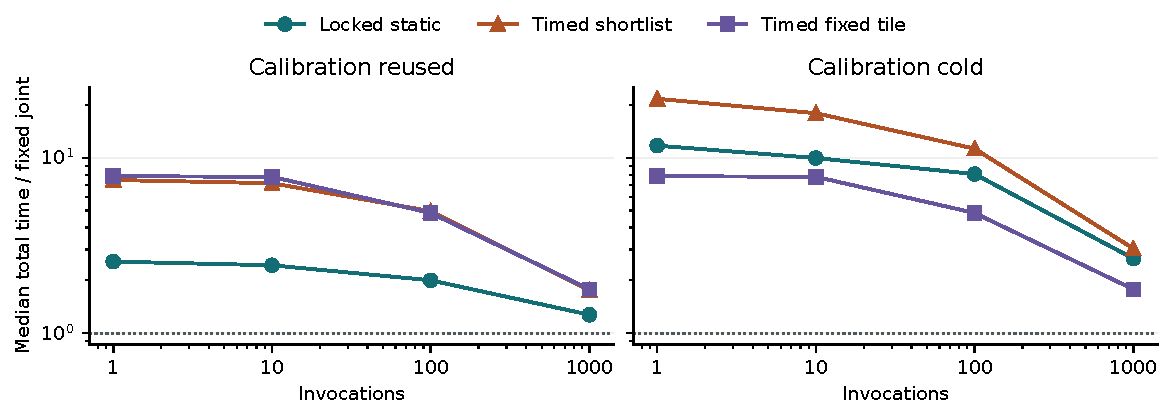
\includegraphics[width=.9\linewidth]{reuse.pdf}
\caption{Per-graph total time divided by the total for fixed joint, summarized by the median over 24 primary graphs. The dotted line marks equality. Both axes use logarithmic scales.}\label{fig:reuse}
\end{figure}

\section{Limitations}
All measurements used one pinned logical CPU, one compiler stack, short inference graphs and fixed weights. The two official ResNet subgraphs establish a limited transfer test. Trained networks, multicore servers and accelerator execution require separate measurements. Even when HLO matches, backend and measurement variation remain possible. One of the 24 one-tile equivalence controls crossed the empirical A/A threshold. Compiler allocation, tagged operation counts and LLVM stores support a mechanism. Isolating cache traffic requires hardware counters. Five external processes and three synthetic confirmation processes also limit estimates of tail variability. The within-case minimum across valid candidates is an optimistic comparator.

The fresh sample includes three sizes per primary family. Its confidence interval describes resampling these size blocks and process repetitions on this machine. The four mixed synthetic graphs test only two ordered compositions. Logical exported bytes and Windows process-cycle counts do not identify memory-controller traffic or instruction counts. GPU launches, device-memory traffic and transfer of a CPU-trained policy to another backend remain open questions.

\section{Conclusion}
The output contract permits optimization even when moving the counters across ReLU produces identical HLO. Main-only controls show that a tile can change the incremental benefit of combining the two reductions. A coefficient-independent dominance test explains why the first cost model missed measured alternatives. Operator and tile interactions allowed the locked replacement to reduce aggregate execution latency on new CPU shapes. Fixed joint retained an advantage on dense and convolution graphs and for most deployments of 1,000 calls or fewer. An evaluation of a selector therefore needs both independent schedule measurements and an explicit invocation horizon.

\paragraph{Artifact availability.}
The \href{https://github.com/ZZzJunzum/Compiler_report/tree/e5964158e339cb1ff866b5f1ca4d0ba3bc9b6325}{versioned experimental archive}
contains the \artifact{protocol.json}{placement protocol},
\artifact{results/phase2/protocol.json}{execution protocol},
\artifact{results/phase2/analysis/PHASE0.md}{HLO and LLVM audit},
\artifact{results/phase2/model/features.csv}{frozen features},
\artifact{results/phase2/model/predictions.csv}{pre-confirmation predictions},
and \artifact{results/phase2/model/heldout_results.csv}{held-out decisions}.
The \href{https://github.com/ZZzJunzum/Compiler_report/tree/a8fd22575ffc293c850b922b95e1feb5e5e68272/results/phase3/cpu/static}{static lock} and the \href{https://github.com/ZZzJunzum/Compiler_report/tree/ed3876906c9431baa2f9465d6449c36d94bd9042/results/phase3/cpu/decision}{discovery lock} precede the \href{https://github.com/ZZzJunzum/Compiler_report/tree/08e3fe6b8ed3e235f175288b1645ca7e3ad9b390/results/phase3/cpu}{Phase III CPU measurements}. Each dispatch, numerical check and compiler listing is indexed by workload, strategy, cohort and process.

\begin{thebibliography}{9}\small
\bibitem{spartan} S. Dong et al. \href{https://doi.org/10.1109/TPDS.2021.3067825}{Spartan: A Sparsity-Adaptive Framework to Accelerate Deep Neural Network Training on GPUs}. \emph{IEEE Transactions on Parallel and Distributed Systems} 32(10), 2448--2463, 2021.
\bibitem{systemml} M. Boehm, B. Reinwald, D. Hutchison, P. Sen, A. V. Evfimievski, and N. Pansare. \href{https://doi.org/10.14778/3229863.3229865}{On Optimizing Operator Fusion Plans for Large-Scale Machine Learning in SystemML}. \emph{Proceedings of the VLDB Endowment} 11(12), 1755--1768, 2018.
\bibitem{xtat} P. M. Phothilimthana et al. \href{https://mangpo.net/papers/xla-autotuning-pact2021.pdf}{A Flexible Approach to Autotuning Multi-Pass Machine Learning Compilers}. \emph{PACT}, 2021.
\bibitem{halide} J. Ragan-Kelley, C. Barnes, A. Adams, S. Paris, F. Durand, and S. Amarasinghe. \href{https://people.csail.mit.edu/jrk/halide-pldi13.pdf}{Halide: A Language and Compiler for Optimizing Parallelism, Locality, and Recomputation in Image Processing Pipelines}. \emph{PLDI}, 2013.
\bibitem{onednn} J. Li et al. \href{https://arxiv.org/abs/2301.01333}{oneDNN Graph Compiler: A Hybrid Approach for High-Performance Deep Learning Compilation}. \emph{CGO}, 2024.
\bibitem{cuda} M. Dodovi\'c, M. Veselinovi\'c, and M. Mi\v{s}i\'c. \href{https://doi.org/10.3390/electronics15051034}{Analyzing the Impact of Kernel Fusion on GPU Tensor Operation Performance: A Systematic Performance Study}. \emph{Electronics} 15(5), 1034, 2026.
\bibitem{roofline} S. Williams, A. Waterman, and D. A. Patterson. \href{https://www2.eecs.berkeley.edu/Pubs/TechRpts/2008/EECS-2008-134.html}{Roofline: An Insightful Visual Performance Model for Floating-Point Programs and Multicore Architectures}. UC Berkeley Technical Report UCB/EECS-2008-134, 2008.
\bibitem{kaufman} S. J. Kaufman, P. M. Phothilimthana, Y. Zhou, C. Mendis, S. Roy, A. Sabne, and M. Burrows. \href{https://proceedings.mlsys.org/paper_files/paper/2021/hash/6bcfac823d40046dca25ef6d6d59cc3f-Abstract.html}{A Learned Performance Model for Tensor Processing Units}. \emph{MLSys}, 2021.
\bibitem{tpugraphs} P. M. Phothilimthana et al. \href{https://proceedings.neurips.cc/paper_files/paper/2023/hash/ded1a89e2b3b925444ada973af66336e-Abstract-Datasets_and_Benchmarks.html}{TpuGraphs: A Performance Prediction Dataset on Large Tensor Computational Graphs}. \emph{NeurIPS}, Datasets and Benchmarks Track, 2023.
\end{thebibliography}
\end{document}
